\documentclass{article}
\usepackage{listings}
\usepackage{hyperref}
\hypersetup{
	 colorlinks   = true,
     citecolor    = black,
     linkcolor    = black,
     urlcolor     = black
}
\usepackage{graphicx}
\usepackage{algorithm}
\usepackage{algpseudocode}
\usepackage{amsmath}
\usepackage{tikz}
\usepackage{caption}
\usepackage{subcaption}
\usetikzlibrary{arrows,matrix,positioning}

\begin{document}
\title{DIP Homework 1}
\author{Qiuyi Zhang 12330402 \\ \href{mailto:joyeec9h3@gmail.com}{joyeec9h3@gmail.com}} 
\date{\today}
\maketitle

\section{Exercises}

\subsection{Storage}
\begin{enumerate}
\item How many bit planes are there for this image?

\textbf{Answer:} There are $\log_{2} 256 = 8$ bit planes.

\item Which plane is the most visually significant one?

\textbf{Answer:} The one that contains the set of the most significant bit -- the 8th plane.

\item How many bytes are required for storing this image? (Don’t consider image headers and compression.)

\textbf{Answer:} 
\begin{align*} 
\textrm{Bytes needed} & = 2048 \times 2048\textrm{ bit per plane} \times 8\textrm{ planes} \\
 & = 2^{22} \times 8\textrm{ bits} \\
 & = 2^{22}\textrm{ bytes}
\end{align*}
\end{enumerate}

\subsection{Adjacency}

\begin{figure}[ht]
\begin{minipage}[b]{0.45\linewidth}
\centering
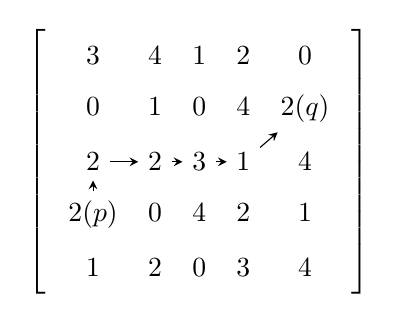
\begin{tikzpicture}
\matrix [matrix of math nodes,left delimiter={[},right delimiter={]}] (m)
{
    3 & [1ex] 4 & [1ex] 1 & [1ex] 2 & [1ex] 0\\[1ex]
    0 & [1ex] 1 & [1ex] 0 & [1ex] 4 & [1ex] 2(q)\\[1ex]
    2 & [1ex] 2 & [1ex] 3 & [1ex] 1 & [1ex] 4\\[1ex]
    2(p) & [1ex] 0 & [1ex] 4 & [1ex] 2 & [1ex] 1\\[1ex]
    1 & [1ex] 2 & [1ex] 0 & [1ex] 3 & [1ex] 4\\[1ex]
};
\path[-stealth] (m-4-1) edge (m-3-1);
\path[-stealth] (m-3-1) edge (m-3-2);
\path[-stealth] (m-3-2) edge (m-3-3);
\path[-stealth] (m-3-3) edge (m-3-4);
\path[-stealth] (m-3-4) edge (m-2-5);
\end{tikzpicture}
\caption{Shortest 4-path a}
\label{fig:32_a}
\end{minipage}
\hspace{0.5cm}
\begin{minipage}[b]{0.45\linewidth}
\centering
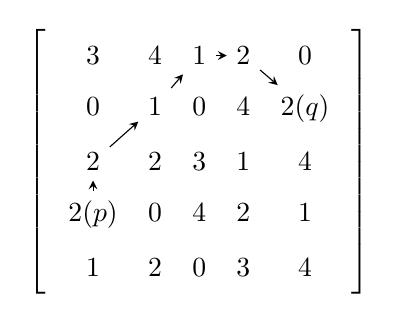
\begin{tikzpicture}
\matrix [matrix of math nodes,left delimiter={[},right delimiter={]}] (m)
{
    3 & [1ex] 4 & [1ex] 1 & [1ex] 2 & [1ex] 0\\[1ex]
    0 & [1ex] 1 & [1ex] 0 & [1ex] 4 & [1ex] 2(q)\\[1ex]
    2 & [1ex] 2 & [1ex] 3 & [1ex] 1 & [1ex] 4\\[1ex]
    2(p) & [1ex] 0 & [1ex] 4 & [1ex] 2 & [1ex] 1\\[1ex]
    1 & [1ex] 2 & [1ex] 0 & [1ex] 3 & [1ex] 4\\[1ex]
};
\path[-stealth] (m-4-1) edge (m-3-1);
\path[-stealth] (m-3-1) edge (m-2-2);
\path[-stealth] (m-2-2) edge (m-1-3);
\path[-stealth] (m-1-3) edge (m-1-4);
\path[-stealth] (m-1-4) edge (m-2-5);
\end{tikzpicture}
\caption{Shortest 4-path b}
\label{fig:32_b}
\end{minipage}
\end{figure}

\end{document}